\documentclass{article}
\usepackage{amsmath}
\usepackage{graphicx}
\usepackage{float}
\usepackage{enumitem}
\pagestyle{empty}
\begin{document}
\section{C - curve}

Given 

\begin{enumerate}
    \item coordinate of inital point A (\(x,y \))
    \item length of inital line \(= len \)
    \item angle \(\alpha\) x-axis with initial line
    \item order \(n\) of the C curve
\end{enumerate}

Now if \(n=0 \) we draw line segment from point A (\(x,y \)) of length \(len \) at angle \(\alpha \) with x - axis. That's our \(0^{th} \) degree C curve.\\
Otherwise if \(n > 0\) then we draw lines of equal length from each endpoints of line segment of \((n-1)^{th}\) degree C curve making angle \(\frac{\pi}{2}\).

\begin{figure}[h]
    \centering
    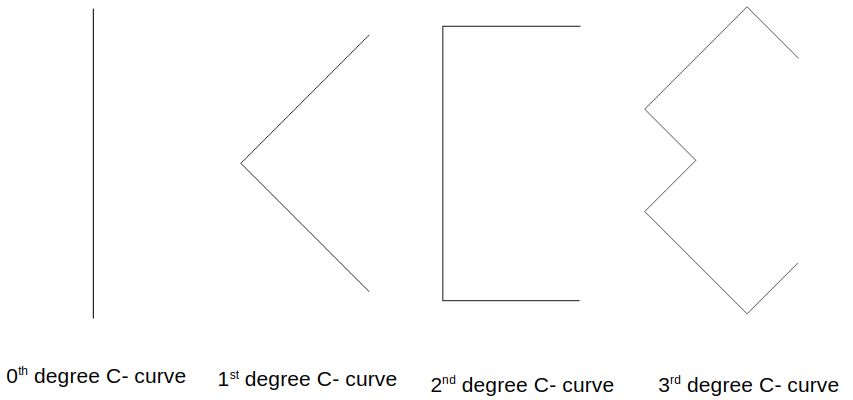
\includegraphics[width=0.9\textwidth]{figures/c0123}
    \caption{Various C curves}
\end{figure}
\subsection{Derivations}

We have an \(\triangle ABC\) whose side \(AB\) make \(\alpha \) with x-axis and \(AC = BC\).
We make following claims and then prove it.

\begin{enumerate}[label=\roman*.,start=1]
    \item \(\angle CAM = \angle CBM = \frac{\pi}{4} \)
    \item \(AC = BC = \frac{len}{\sqrt{2}}\)
\end{enumerate}

\begin{figure}[H]
    \centering
    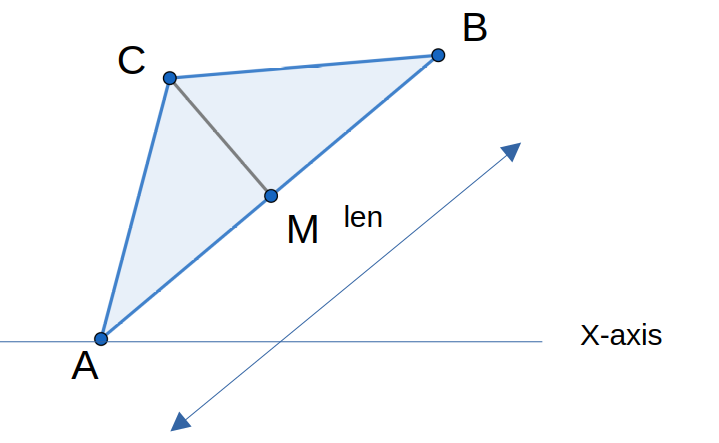
\includegraphics[width=
    0.9\textwidth]{figures/fig1}
    \caption{For proving elementry properties}
\end{figure}

For i. \\
We join line from C to M.\\
\(\triangle ABC\) is an isosceles as \(AC = BC \). \\
\(\Rightarrow \angle CAM = \angle CBM \)\\
Also, in \(\triangle ABC\)

\begin{align*}
    \angle CAM + \angle CBM +\angle ACB &= \pi \\
   2 \angle CAM + \angle ACB &= \pi \\
   2 \angle CAM &= \frac{\pi}{2} \left[\text{ Since }  \angle ACB = \frac{\pi}{2}  \right]\\
   \angle CAM &= \frac{\pi}{4} = \angle CBM 
\end{align*}

i. is proved. 

For ii. \\
We draw a line from C to mid point M of AB. \\
Consider \(\triangle CAM\) and \(\triangle CBM \). \\
Clearly, 

\begin{align*}
    CA &= CB \\
    \angle CAM &= \angle CBM \\
    AM &= BM
\end{align*}

By SAS criterion,

\begin{align*}
    \triangle CAM \cong \triangle CBM  \\
    \Rightarrow \angle ACM = \angle BCM 
\end{align*}

But, 

\begin{align*}
    \angle ACB &= \frac{\pi}{2}\\
    \angle ACM + \angle BCM &= \frac{\pi}{2} \\
    2 \angle ACM &= \frac{\pi}{2} \\
    \angle ACM &= \frac{\pi}{4} = \angle BCM
\end{align*}

So, 


\( \triangle ACM \) and \( \triangle BCM \) are also isosceles.\\
\( \Rightarrow AM = MC = MB = \frac{len}{2} \)


Consider \(\triangle ACM ,\) 

\begin{align*}
   AM^2 + CM^2 &= AC^2 \left[ \text{ Since, } \angle AMC = \frac{\pi}{2} \right] \\
   \frac{len}{4}^2 + \frac{len}{4}^2 &= AC^2 \left[ \text{  Since, M is mid point of AB}\right]\\
   AC &= \frac{len}{\sqrt{2}} = BC \left[\triangle ABC \text{  is isosceles}\right]
\end{align*}
ii. is also proved.

Now, we make few more claims and then prove them.

\begin{enumerate}[label=\roman*.,start=3]
    \item \(B (a, b) \equiv (x+len \cos \alpha, y + len \sin \alpha)\)
    \item \(C (x', y') \equiv \left(x+\frac{len }{\sqrt{2}} \cos (\alpha + \frac{\pi}{4}), y + \frac{len}{\sqrt{2}} \sin (\alpha + \frac{\pi}{4})\right)\)
    \item \(B (a, b) \equiv \left(x' +\frac{len }{\sqrt{2}} \cos (\alpha - \frac{\pi}{4}), y' + \frac{len}{\sqrt{2}} \sin (\alpha - \frac{\pi}{4})\right)\)
\end{enumerate}

\begin{figure}[H]
    \centering
    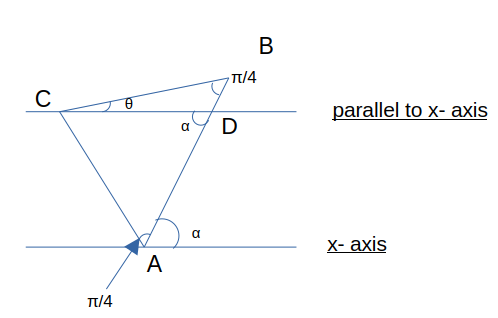
\includegraphics[width=
    0.9\textwidth]{figures/fig2}
    \caption{For proving core properties}
\end{figure}

For iii. We have,

\begin{align*}
    \cos \alpha &= \frac{a-x}{len}\\
    a &= x + len \cos \alpha\\
\end{align*}

Similarly,

\begin{align*}
    \sin \alpha &= \frac{b-y}{len}\\
    b &= y +len \sin \alpha
\end{align*}

Thus,

\begin{align*} 
    (a, b) \equiv (x+len \cos \alpha, y + len \sin \alpha)
\end{align*}

For iv. We can clearly see that angle made by AC with x-axis is \(\frac{\pi}{4}\). By same procedure as above, we arrive at

\begin{align*}
    \cos \left(\alpha + \frac{\pi}{4}\right) &= \frac{x'-x}{\frac{len}{\sqrt{ 2}}}\\
    x' &= x + \frac{len}{\sqrt{2}} \cos\left(\alpha + \frac{\pi}{4})\right)
\end{align*}

    And, 

\begin{align*}
    \sin \left(\alpha + \frac{\pi}{4}\right) &= \frac{y'-y}{\frac{len}{\sqrt{ 2}}}\\
    y' &= y + \frac{len}{\sqrt{2}} \sin \left(\alpha + \frac{\pi}{4}\right)\\
\end{align*}

    Thus, 

\begin{align*}
(x', y') \equiv \left(x+\frac{len }{\sqrt{2}} \cos (\alpha + \frac{\pi}{4}), y + \frac{len}{\sqrt{2}} \sin (\alpha + \frac{\pi}{4})\right)
\end{align*}

For v. We will only show that \(\theta = \alpha - \frac{\pi}{4}\) which is quite clear from fig. 3 and rest of the procedure is left to the reader as it is similar.

\begin{align*}
    \angle CDA = \alpha \left[\text{ Since, CD is parallel to x-axis}\right]\\
\end{align*}

So, 

\begin{align*}
    \angle BCD + \angle CBD + \angle CDB &= \pi\\
    \theta + \frac{\pi}{4} + (\pi - \alpha) &= \pi\\
    \theta &= \alpha - \frac{\pi}{4}
\end{align*}

By ditto procedure, we get

\begin{align*}
    (a, b) \equiv \left(x' +\frac{len }{\sqrt{2}} \cos (\alpha - \frac{\pi}{4}), y' + \frac{len}{\sqrt{2}} \sin (\alpha - \frac{\pi}{4})\right)
\end{align*}

\subsection{Pseudocode}
C-curve (\(x \, y \, len \, \alpha \, n\))

\begin{enumerate}
    \item if \(n=0\) \begin{enumerate}
        \item draw line between \((x, y)\) and \((x+len \cos \alpha, y + len \sin \alpha)\) i.e from A to B
    \end{enumerate}
    \item if \(n > 0\) \begin{enumerate}
        \item C-curve (\(x \, y \, \frac{len}{\sqrt{2}} \, (\alpha + \frac{\pi}{4}) \, (n-1)\)) i.e. draw C curve from A toward C, reducing degree by 1
        \item Compute \(C (x', y') \equiv \left(x+\frac{len }{\sqrt{2}} \cos (\alpha + \frac{\pi}{4}), y + \frac{len}{\sqrt{2}} \sin (\alpha + \frac{\pi}{4})\right)\)
        \item C-curve (\(x' \, y' \, \frac{len}{\sqrt{2}} \, (\alpha - \frac{\pi}{4}) \, (n-1)\)) i.e. draw C curve from C toward B reducing degree by 1
    \end{enumerate}
\end{enumerate}

\begin{figure}[H]
    \centering
    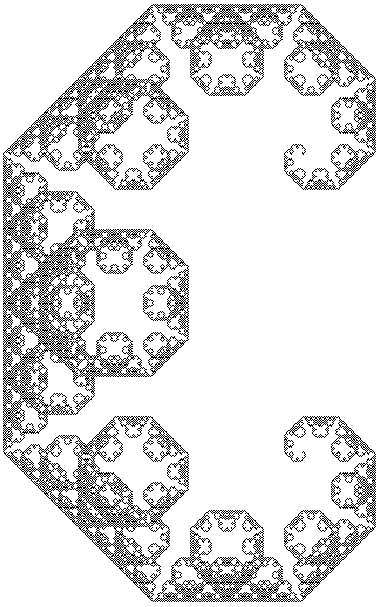
\includegraphics[scale=0.4]{figures/c15}
    \caption{\(15^{th}\) degree C curve}
\end{figure}

\end{document}